\documentclass[12pt]{article}


\usepackage{graphicx}
\usepackage{colortbl}
\usepackage{xr}
\usepackage{longtable}
\usepackage{xfrac}
\usepackage{tabularx}
\usepackage{booktabs}
\usepackage{hyperref}
\usepackage{xcolor} % for different colour comments
\usepackage{fullpage}
\newcounter{rowcount}
\setcounter{rowcount}{0}


\hypersetup{
    bookmarks=true,         % show bookmarks bar?
      colorlinks=true,       % false: boxed links; true: colored links
    linkcolor=black,          % color of internal links (change box color with linkbordercolor)
    citecolor=green,        % color of links to bibliography
    filecolor=magenta,      % color of file links
    urlcolor=cyan           % color of external links
}

%% Comments
\newif\ifcomments\commentstrue
\ifcomments
\newcommand{\authornote}[3]{\textcolor{#1}{[#3 ---#2]}}
\newcommand{\todo}[1]{\textcolor{red}{[TODO: #1]}}
\else
\newcommand{\authornote}[3]{}
\newcommand{\todo}[1]{}
\fi
\newcommand{\wss}[1]{\authornote{magenta}{SS}{#1}}
\newcommand{\ds}[1]{\authornote{blue}{DS}{#1}}
\newcommand{\kly}[1]{\authornote{green}{KL}{#1}}
\newcommand{\cc}[1]{\authornote{orange}{CC}{#1}}

%%%%%%%%%%%%%%%%%%%%%%%%%%%%%

\begin{document}

\title{Test Plan for Quarters} 
\author{James Anthony (anthonjb)\\ Wenqiang Chen (chenw25)\\ Carolyn Chong 
(chongce)\\ Kevin Ly (lyk2)}
\date{\today}
  
\maketitle

\pagebreak

\tableofcontents

\section*{Revision History}
\begin{tabular}{|c|c|}
\hline
\textbf{Date}  & \textbf{Comments} \\ \hline
October 21, 2015 & Created first draft. \\ 
\hline
March 20, 2016 & Removed Chat system tests, updated test case numbers and Usability section. \\ 
\hline
\end{tabular}

\section*{Template}
This document makes use of the Validation, Verification and Testing Plan Template, and "Integrated Stroke Test Plan" for all of its organization.

\ds{A brief introduction or system description would be useful.}

\pagebreak

%%%%%%%%%%%%%%%%%%%%%%%%%%%%%

%Acronyms and Definitions
\section{Acronyms and Definitions}
\renewcommand{\arraystretch}{1.2}
\begin{tabular}{l l} 
  \toprule    
  \textbf{Acronym} & \textbf{Description}\\
  \midrule 
  PoC   &Proof of Concept\\
  \bottomrule
\end{tabular}\\


%Plans for Automated Testing
\section{Plans for Automated Testing}
All tests that will be automated will be completed for the Final Demo April 1. We will automate testing for every feature, except financing, notification and chat. We will also test the integrity of the database using automated testing. We will also check if every page is reachable, to ensure there are no unhandled HTTP errors. We plan to run automated tests on a weekly basis, every Sunday night. Automated testing tools include Grunt, SinonJS and custom Python scripts. 

%Plans for Unit Testing
\section{Plans for Unit Testing}
All unit tests will be automated. Unit tests will be created as features are developed. They will be separated by module. Since the majority of modules will be Javascript, we will be using QUnit. QUnit is a Javascript unit testing framework. 

\ds{You should start planning your unit tests now. You can determine the
majority of them ahead of time.}

%System Tests
\section{System Tests}

%4.1 User Registration
\subsection{User Registration} 
\textbf{Test Type:} Functional, Dynamic, Automated. \\
\textbf{Tools Used:} Custom Scripts, Google reCAPTCHA. \\
\textbf{Schedule:} Begin testing November 8. Complete manual tests by PoC Demo November 16. Complete automated dynamic tests by Final Demo April 1. \\
\textbf{Team Member Responsible:} Carolyn Chong.\\
\textbf{Methodology:} The main objective of user registration is to create a user account to be used for login. Users must use a valid email address and pass a user identification procedure. This ensures the user is human and prevents spam and automated scripts from accessing the application and abusing its services. Testing is manual and automated. Manual testing involves people manually going through the registration process in real-time as a user. Automated testing involves systemically attempting SQL injections to test for valid and invalid registrations. Google reCAPTCHA validates that users are legitimate.

\begin{longtable}{|p{2cm}|p{3cm}|p{5cm}|p{5cm}|}
\hline
\textbf{Test Case}  & \textbf{Initial State} & \textbf{Input} & \textbf{Output} \\ \hline
1.1 & Landing page. Empty fields. & Email and password entered and passes reCAPTCHA test. Clicks register. & Verification email sent. Redirected to application main page. \\ 
\hline
1.2 & Landing page. Empty fields. & Empty field(s). Clicks register. & Stays on the same page. Error message appears. Empty field is highlighted. \\
\hline
1.3 & Landing page. Empty fields. & Email address already stored in database. Clicks register. & Stays on the same page. Error message appears. Email field is highlighted. \\
\hline
1.4 & Landing page. Empty fields. & Fails reCAPTCHA test. & Stays on the same page. Error message appears. Test field is highlighted. \\
\hline
\end{longtable}



%4.2 User Login
\subsection{User Login}
\textbf{Test Type:} Functional, Dynamic, Automated. \\
\textbf{Tools Used:} Custom Scripts. \\
\textbf{Schedule:} Begin testing November 8. Complete manual tests by PoC Demo November 16. Complete automated dynamic tests by Final Demo April 1. \\
\textbf{Team Member Responsible:} Carolyn Chong. \\
\textbf{Methodology:} The main objective of user login is to ensure a secure process where only valid users are allowed to enter the application. Testing involves authenticating users against an existing database to determine if they are valid users or not. Testing is automated. Automated testing involves systemically attempting SQL injections to test for valid and invalid logins.

\begin{longtable}{|p{2cm}|p{3cm}|p{5cm}|p{5cm}|}
\hline
\textbf{Test Case}  & \textbf{Initial State} & \textbf{Input} & \textbf{Output} \\ \hline
2.1 & Landing page. Empty username and password fields. & Valid username and password combination. Clicks login. & Redirected to application main page. \\ 
\hline
2.2 & Landing page. Empty username and password fields. & Invalid username and password combination. Clicks login. & Stays on the same page. Error message appears. Fields are highlighted. After 5 unsuccessful attempts, user cannot login for 10 minutes. \\
\hline
2.3 & Landing page. Empty username and password fields. & Empty username and/or password fields. Clicks login. & Stays on the same page. Error message appears. Fields are highlighted. \\
\hline
2.4 & Application main page. & Clicks logout. & User is successfully logged out from system. Redirected to login page. \\
\hline
2.5 & Landing page. Empty username and password fields. User attempting to login on another device while already logged in on a device. & Valid username and password combination. Clicks login. & Stays on the same page. Error message appears. \\ 
\hline
\end{longtable}



%4.3 Calendar
\subsection{Calendar}
\textbf{Test Type:} Functional, Dynamic, Automated. \\
\textbf{Tools Used:} Custom Scripts. \\
\textbf{Schedule:} Begin testing after the PoC Demo. Complete automated tests by Final Demo April 1. \\
\textbf{Team Member Responsible:} Carolyn Chong. \\
\textbf{Methodology:} The Calendar feature allows users to add/delete events and chores to a shared Calendar between members of a house. This shared Calendar can be synched with a user's personal Calendar. Testing is automated. Automated testing involves a script that will go through the process of adding/deleting an event or chore to the Calendar in real-time as a user, and then checking if those updates are properly synched with the user's personal Calendar. 

\begin{longtable}{|p{2cm}|p{3cm}|p{5cm}|p{5cm}|}
\hline
\textbf{Test Case}  & \textbf{Initial State} & \textbf{Input} & \textbf{Output} \\ \hline
3.1 & Calendar page. & Select date. & Form opens. \\ 
\hline
3.2 & Calendar page. Existing form is open. & User modifies event details and saves changes. & Form closes and updated Calendar is displayed. \\ 
\hline
3.3 & Calendar page. Empty form. & Add event/chore. Text entered in fields and saves. & Form closes. Event/chore is updated on Calendar. \\ 
\hline
3.4 & Calendar page. Empty form. & Add event/chore. Empty field(s). Clicks save. & Form remains open. Error message appears. Empty fields are highlighted. \\
\hline
3.5 & Calendar page. & Click to delete event/chore. & Event/chore is no longer displayed on Calendar. \ds{Who can delete events/chores?} \\
\hline
\end{longtable}

%4.4 Maintenance Ticketing System
\subsection{Maintenance Tracking}
\textbf{Test Type:} Functional, Dynamic, Static, Automated. \\
\textbf{Tools Used:} QUnit, Chron Scripts. \ds{Chron scripts?}\\
\textbf{Schedule:} Begin testing after the PoC Demo. Complete automated tests by Final Demo April 1. \\
\textbf{Team Member Responsible:} Kevin Ly. \\
\textbf{Methodology:} The maintenance tracking system allows tenants to create maintenance requests, where the landlord then responds and updates with further information. This portion of the system is restricted based on the user type; tenants cannot modify maintenance ticket properties. This component will be tested using unit tests for functionality, with automated testing to ensure the permissions are handled properly. Static database checkers will be used in conjunction with the automated test cases to check for proper database modifications.

\begin{longtable}{|p{2cm}|p{3cm}|p{5cm}|p{5cm}|}
\hline
\textbf{Test Case}  & \textbf{Initial State} & \textbf{Input} & \textbf{Output} \\ \hline
4.1 & Quarters Web Application. & Open maintenance system. & Maintenance system opens and shows new maintenance tickets with existing tickets in chronological order. \\ 
\hline
4.2 & Maintenance System. & Click on maintenance ticket. & Inner dialog opens displaying all properties in a maintenance ticket. \\
\hline
4.3 & Maintenance System. & Entering a search query or adding a filter. & Sort and filter maintenance tickets and reveal only successful tickets. \\
\hline
4.4 & Maintenance Ticket Window. & Modifying properties of a ticket. & Save icon appears in dialog to confirm changes.\\
\hline
4.5 & Maintenance Ticket Window. & Saving ticket properties & Window will close, and database will be updated to reflect changes.\\
\hline
4.6 & Maintenance Ticket Window. & Deleting Ticket. & Confirmation window will appear. Upon deletion confirmation, close window and remove data from database.\\
\hline
4.7 & Maintenance System & Click on create new request. & Opens a new ticket window.\\
\hline
4.8 & New Maintenance ticket window. & Click on create empty fields. & Window will remain opening, prompt will display error message.\\
\hline
4.9 & New Maintenance ticket window. & Click on create, required fields filled. & Window closes, database will be updated with new ticket.\\
\hline
4.10 & New Maintenance ticket window. & Click on cancel with fields filled. & Window remains open, prompt will ask for confirmation on close.\\
\hline
4.11 & Confirmation Prompt. & Click on OK. & Closes prompt and dialog. \\
\hline
4.12 & Confirmation Prompt. & Click on cancel. & Closes prompt, dialog remains open.\\
\hline
\end{longtable}

%4.5 house management
\subsection{House Management}
\textbf{Test Type:} Functional, Dynamic, Automated. \\
\textbf{Tools Used:} QUnit. \\
\textbf{Schedule:} Begin testing after the PoC Demo. Complete automated tests by Final Demo April 1. \\
\textbf{Team Member Responsible:} Kevin Ly.\\
\textbf{Methodology:} The house management system allows users to create, delete, view, and modify information about houses. Unit tests will be created for each function in the feature which will be included in the automated testing sequence.

\begin{longtable}{|p{2cm}|p{3cm}|p{5cm}|p{5cm}|}
\hline
\textbf{Test Case}  & \textbf{Initial State} & \textbf{Input} & \textbf{Output} \\ \hline
5.1 & House Management, not admin. & Click modify information. & Nothing.\\ 
\hline
5.2 & House Management, admin. & Click modify information. & Input fields become editable. \\
\hline
5.3 & House Management, admin. & Modify information fields. & Save button opens, discard changes appears. \\
\hline
5.4 & House Management, any user. & Click on View Documents. & Redirects to new page showing all uploaded documents in House. \\
\hline
5.5 & House Documents, any user. & Clicks on a document. & Retrieves documents and initiates file transfer.\\
\hline
5.6 & House Documents, admin. & Clicks on Add Documents. & Upload window opens for user upload, file will be transfer to server and information is updated in database.\\
\hline
5.7 & House Documents, admin. & Clicks on delete document. & Prompt opens.\\
\hline
5.8 & Deletion prompt, admin. & Clicks on yes. & Prompt closed, file is removed from display, database is updated.\\
\hline
5.9 & Deletion prompt, admin. & Clicks on no. & Prompt closed.\\
\hline
5.10 & House Management, any user. & Clicks on view members. & Shows all memebers of the house and their role.\\
\hline
5.11 & House Management, admin, members list visible. & Clicks on add member. & Dialog will appear.\\
\hline
5.12 & Member Dialog, admin, fields empty. & Clicks on ok. & Prompt opens, notifying missing fields. \\
\hline
5.13 & Member Dialog, admin, fields complete. & Clicks on ok. & Window closes, new user is notified, database is updated, member status pending.\\
\hline
5.14 & Member Dialog, admin. & Clicks on cancel. & Window closes.\\
\hline
\end{longtable}

%4.6 landing page
\subsection{Landing Page}
\textbf{Test Type:} Functional, Dynamic, Static, Automated. \\
\textbf{Tools Used:} Custom scripts. \\
\textbf{Schedule:} Begin testing November 8. Complete manual tests by PoC Demo November 16. Complete automated dynamic tests by Final Demo April 1. \\
\textbf{Team Member Responsible:} Kevin Ly.\\
\textbf{Methodology:} The landing page allows users to login and create new accounts. This page also displays information about the application for visitors. This feature will be manually tested since there are not many test cases.

\begin{longtable}{|p{2cm}|p{3cm}|p{5cm}|p{5cm}|}
\hline
\textbf{Test Case}  & \textbf{Initial State} & \textbf{Input} & \textbf{Output} \\ \hline
6.1 & Landing Page, not logged in. & Clicks on login. & Username field appears, password field appears.\\
\hline
6.2 & Landing Page, not logged in. & Clicks on registration. & Email and password fields appear.\\
\hline
\end{longtable}

\ds{So how does registration work? What happens if someone tries to register an existing email/username?}

%4.7 Finance
\subsection{Finance}
\textbf{Test Type:} Functional, Dynamic, Manual. \\
\textbf{Tools Used:} None. \\
\textbf{Schedule:} Begin testing after the PoC Demo. Complete automated tests by Final Demo April 1. \\
\textbf{Team Member Responsible:} James Anthony. \\
\textbf{Methodology:} Tests can be performed by having one user add payment deadlines, and having another user send arbitrary amounts of money via PayPal. Speed and accuracy of transactions can be tracked. Transaction records can be manually evaluated for correctness.

\begin{longtable}{|p{2cm}|p{3cm}|p{5cm}|p{5cm}|}
\hline
\textbf{Test Case} & \textbf{Initial State} & \textbf{Input} & \textbf{Output} \\ \hline
7.1 & No payments due. & User initiates PayPal transaction. & Error message indicating that no payments are due at the current time.\\
\hline
7.2 & No payments due. & User posts payment request with some deadline. & New payment deadline added.\\
\hline
7.3 & Payment due. & User initiates PayPal transaction. & Transaction is handled by PayPal. All users involved are notified of the completed payment. Deadline is removed from list of current payments due.\\
\hline
7.4 & Payment due. & Payment has not been completed, and deadline has passed. & All users involved are notified that the deadline has passed. Deadline is marked as past due, and users will continue to be notified until either the payment has been completed, or the due payment is removed.\\
\hline
7.5 & Payment due. & User who posted the original due payment removes the request. & Payment request is removed from the list of due payments.\\
\hline
\end{longtable}


%4.8 Notification
\subsection{Notifications}
\textbf{Test Type:} Functional, Dynamic, Manual. \\
\textbf{Tools Used:} None. \\
\textbf{Schedule:} Begin testing after the PoC Demo. Complete automated tests by Final Demo April 1. \\
\textbf{Team Member Responsible:} Wenqiang Chen. \\
\textbf{Methodology:} The main objective of notification is to remind user of events that has had happened; users should be notified immediate after the event has taken place. The testing involves one user completing different actions which generates notification and have another user related to this event receive notification.

\begin{longtable}{|p{2cm}|p{3cm}|p{5cm}|p{5cm}|}
\hline
\textbf{Test Case}  & \textbf{Initial State} & \textbf{Input} & \textbf{Output} \\ \hline
8.1 & Main page. User(A) logged in. & User(B) sends money request. & User(A) sees notification of pending payment due.  \\ 
\hline
8.2 & Main page. User(A) logged in. & User(A) pays user(B). & User(B) sees notification of payment completed.  \\ 
\hline
8.3 & Main page. User(A) logged in. & User(A) has late payment. & User(A) sees notification of late payment.  \\ 
\hline
8.4 & Main page. User(A) logged in. & User(A) joins a house.  & Other users in that house sees notification that user(A) joined the house. \\
\hline
8.5 & Main page. User(A)(landlord) logged in. & User(B) sends maintenance ticket(Critical). & User(A) sees notification of unresolved maintenance ticket, receives email, receives text message. \\
\hline
8.6 & Main page. User(A)(landlord) logged in. & User(B) sends maintenance ticket(Major.) & User(A) sees notification of unresolved maintenance ticket, receives email.\\
\hline
8.7 & Main page. User(A)(landlord) logged in. & User(B) sends maintenance ticket(Minor). & User(A) sees notification of unresolved maintenance ticket. \\
\hline
8.8 & Main page. User(A) logged in. & User(B)(Landlord) resolves a maintenance ticket. & User(A) sees notification of resolved maintenance ticket. \\
\hline
8.9 & Main page. User(A) logged in. & User(B) sends user(A) a message. & User(A) sees notification of unread message. \\
\hline
8.10 & Main page. User(A) logged in. & User(B) makes a post in discussion board. & User(A) sees notification of unread post. \\
\hline
8.11 & Main page. User(A) logged in. & User(B) replies to a post made by user(A). & User(A) sees notification of unread reply. \\
\hline
8.12 & Main page. User(A) logged in. & User(A) leaves a house.  & Other users in that house sees notification that user(A) left the house. \\
\hline
8.13 & Main page. User(A) logged in. & User(B) adds event to Calendar. & User(A) sees notification of added post. \\
\hline
8.14 & Main page. User(A) logged in. & User(B) deletes event from Calendar. & User(A) sees notification of deleted event. \\
\hline
8.15 & Main page. User(A) logged in. & User(A)has event happening on day. & User(A) sees notification of event. \\
\hline
8.16 & Main page. User(A) logged in. Notification displayed. & User clicks on Notification icon. & Notification disappears. \\
\hline
\end{longtable}

%4.9 Administrative File Storage
\subsection{Administrative File Storage}
\textbf{Test Type:} Functional, Dynamic, Automated. \\
\textbf{Tools Used:} Custom Scripts. \\
\textbf{Schedule:} Begin testing after the PoC Demo. Complete automated tests by Final Demo April 1. \\
\textbf{Team Member Responsible:} James Anthony. \\
\textbf{Methodology:} A script can be used to test the process of uploading and downloading multiple files of different types and sizes.

\begin{longtable}{|p{2cm}|p{3cm}|p{5cm}|p{5cm}|}
\hline
\textbf{Test Case} & \textbf{Initial State} & \textbf{Input} & \textbf{Output} \\ \hline
9.1 & 0 files in storage. & User tries to upload a file of size $s$, where $s \le$ max file size. & Successful file upload.\\
\hline
9.2 & 0 files in storage. & User tries to upload a file of size $s$, where $s >$ max file size. & Error message indicating file has not been uploaded.\\
\hline
9.3 & $n$ files in storage. & User tries to upload a file of size $s$, where $s \le$ total remaining space. & Successful file upload.\\
\hline
9.4 & $n$ files in storage. & User tries to upload a file of size $s$, where $s >$ total remaining space. & Error message indicating file has not been uploaded.\\
\hline
9.5 & $n$ files in storage. & User tries to upload a file with an invalid type. & Error message indicating file has not been uploaded.\\
\hline
9.6 & $n$ files in storage. & User requests to download a file. & Successful file download.\\
\hline
9.7 & $n$ files in storage. & Connection interrupted while download is in progress. & Error message indicating file has not been downloaded.\\
\hline
9.8 & $n$ files in storage. & User tries to upload  $n > 1$ files. & Error message indicating only one file can be uploaded at a time.\\
\hline
9.9 & $n$ files in storage. & User clicks delete file. & File removed. \\
\hline
\end{longtable}

%4.10 Bulletin Board
\subsection{Bulletin Board}
\textbf{Test Type:} Functional, Dynamic, Automated. \\
\textbf{Tools Used:} Custom Scripts. \\
\textbf{Schedule:} Begin testing after the PoC Demo. Complete automated tests by Final Demo April 1. \\
\textbf{Team Member Responsible:} James Anthony. \\
\textbf{Methodology:} A script can be used to test the process of posting on the discussion board, and commenting on existing posts.

\begin{longtable}{|p{2cm}|p{3cm}|p{5cm}|p{5cm}|}
\hline
\textbf{Test Case} & \textbf{Initial State} & \textbf{Input} & \textbf{Output} \\ \hline
10.1 & No posts on bulletin board. & A post with 0 characters & Empty post is disgarded
\ds{``discarded"}
and not added to bulletin board.\\
\hline
10.2 & No posts on bulletin board. & A post with $n$ characters, where $n > 0$. & Bulletin board is updated with the post of $n$ characters.\\
\hline
10.3 & $p$ posts on bulletin board, where $p > 0$. & A post with 0 characters & Empty post is disgarded and not added to bulletin board.\\
\hline
10.4 & $p$ posts on bulletin board, where $p > 0$. & A post with $n$ characters, where $n > 0$. & Bulletin board is updated with the post of $n$ characters.\\
\hline
10.5 & $p$ posts on bulletin board, where $p > 0$. & A comment with 0 characters on an existing post $p$. & Empty comment is disgarded
\ds{discarded}
and not added to bulletin board.\\
\hline
10.6 & $p$ posts on bulletin board, where $p > 0$. & A comment with $n$ characters where $n > 0$, on an existing post $p_i$. & Comment is added to the list of comments associated with post $p_i$.\\
\hline
\end{longtable}


%5. Non-Functional Tests
\section{Non-Functional Tests}

\subsection{Usability}
This section describes a test plan for conducting a usability test for the Quarters application. 

\subsubsection{Participants}
The participants' responsibilities were to attempt to complete a set of representative task scenarios presented to them in as efficient and timely a manner as possible, and to provide feedback regarding the usability and acceptability of the user interface.  The participants were directed to provide honest opinions regarding the usability of the application, and to participate in a post-session subjective questionnaire.\\ \\
Eight participants, who were tenants themselves, were selected from Thode library at McMaster University. Four females and four males participated as tenants. They were between the ages of 18-22 years old. Participants were recruited by approaching students during day-time hours while they were studying. We recruited participants who were willing to use either their personal laptop or mobile device and run the application on their web browser. Participants were given a background on the project and were told the methodology of the test. Participants were then asked if they would volunteer their time to participate. No certain skills and/or background were required, however, it was expected that participants were familiar with using a web browser on a computer. Additionally, two participants, who were landlords themselves, were approached and selected by Quarters developers as they were the current landlords of the developers.

\subsubsection{Training}
The participants received an overview of Quarters and written instructions of the usability test procedure. No training was delivered on how to use Quarters; only a link to the landing page was given. The test environment was that of where the user was located at the time of recruitment, since that was most convenient for participants. All tenant participants took the test seated at a table on the first floor of Thode library. The first floor of Thode Library is known to be loud relative to a typical library setting. All participants were surrounded by non-participants talking at a conversational noise level. The library was considered ‘busy’, as every seat at every table was occupied at the time of testing. Landlord participants took the test at the rental house, also seated, but in a quieter setting relative to the library.

\subsubsection{Procedure}
The participants used their own laptop or mobile device to complete the usability test. The only requirement was that they completed the test on either Chrome, Opera, Explorer, Firefox, or Safari. The participant’s interaction with Quarters was monitored by the facilitator seated beside the participant. \\ \\
The facilitator briefed the participants on Quarters and instructed the participant that they were evaluating the application, rather than the facilitator evaluating the participant. Participants were informed that participation was voluntary and that participation could cease at any time. The facilitator asked the participant if they had any questions. \\ \\
Participants completed a pretest demographic and background information questionnaire as part of Task 1. Then, the facilitator explained that the amount of time taken to complete the test task would be measured. Participants were instructed that exploratory behavior outside the task flow should not occur. At the start of each task, the participant read aloud the task description from the printed copy and began the task. Time-on-task began when the participant started each task. \\ \\
The facilitator instructed the participant to ‘think aloud’ so that a verbal record existed of their interaction with Quarters. The facilitator observed and recorded user behaviour and user comments in a text editor. \\ \\
Task 2a required the landlord participants to create an account, login, create a house, and then create a post on the bulletin board. The facilitator explained that the number of button clicks and the amount of time taken to complete the test task would be measured. \\ \\
Task 2b required the tenant participants to create an account, login, and then create a post on the discussion board. The facilitator explained that the number of button clicks and the amount of time taken to complete the test task would be measured. \\ \\
After all task scenarios were attempted, the participant completed the post-test satisfaction questionnaire as part of Task 3. 
Due to the range and extent of functionality provided in the application, and the short time for which each participant was available, the tasks were the most common and relatively complex of available functions. Furthermore, the tasks represent a high-level goal of the software, that is, the ability to effectively and efficiently communicate. The tasks were identical for all participants in each subset in the study. \\ \\
A sample of the usability test instructions and questionnaires given to participants is in the Appendix, labelled Figure \ref{fig:test}. 

\subsubsection{Success Metrics}
Success metrics were guided by task completion success rates, task completion times, and subjective evaluations.
Completion rate was the percentage of test participants who successfully completed Task 2. In other words, the completion rate represented the percentage of participants who, when they were finished with the specified task, had an output that was correct. If a participant required assistance in order to achieve a correct output then the task would not be scored as completed. A completion rate of 100\% was the goal for Task 2 in this usability test.\\ \\ 
Task completion time was the time to complete the task.  It was measured from the time the person began the task to the time he/she signaled completion. An average task completion time of less than 60 seconds was the goal for the task in this usability test. \\ \\
Subjective evaluations regarding ease of use and satisfaction were collected via a questionnaire.  The questionnaire utilized rating scales. This data was used to assess attitudes of the participants.


\subsection{Performance}
To test the server, we will do a load testing to make sure the server can handle 100 simultaneous requests.

\ds{How?}

\subsection{Security}
To test the security of the system, including file access, failed password attempts, SQL injections, and expired sessions, we will do manual testing.

\ds{Be more descriptive.}

\section{Appendix}
\begin{figure}[h]
    \centering
    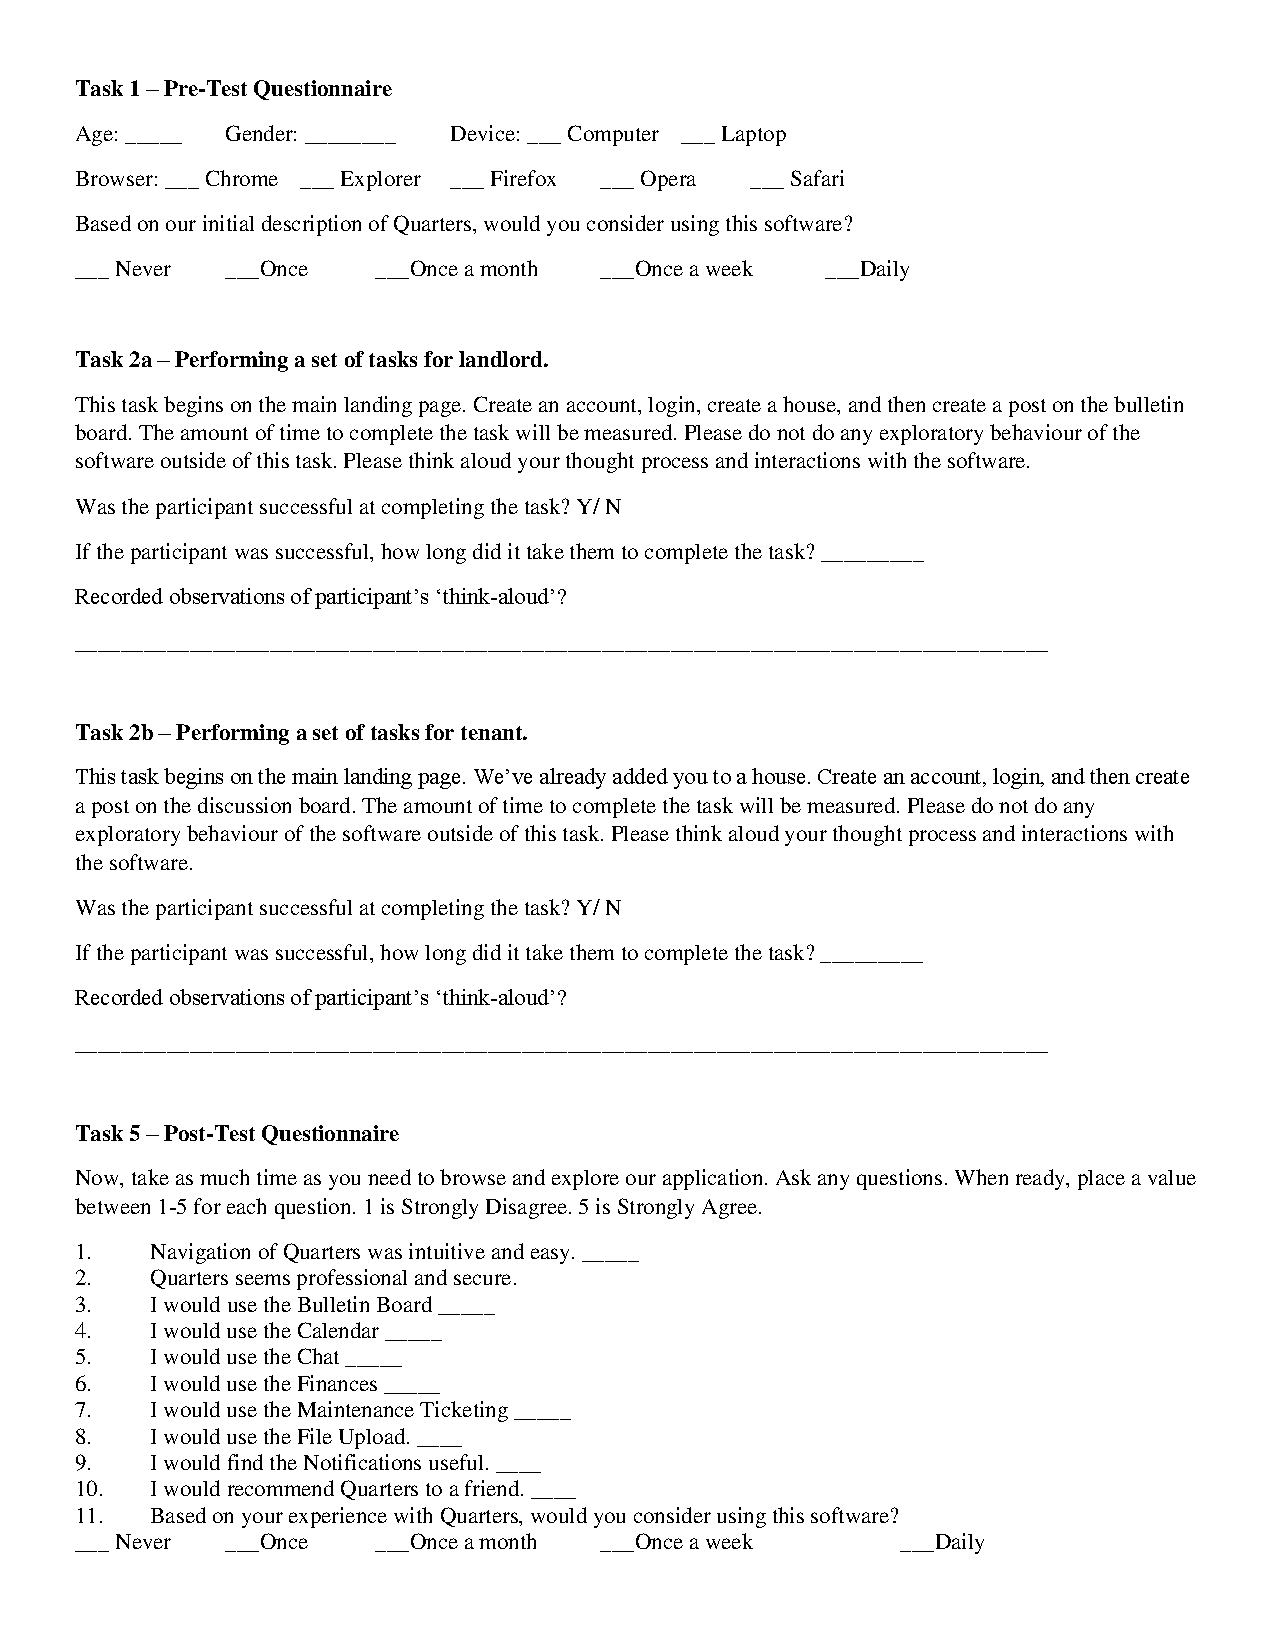
\includegraphics[width=1\textwidth]{usabilityTest.pdf}
    \caption{Sample Usability Test Questionnaire}
    \label{fig:test}
\end{figure}


\end{document}
